%
% Copyright (c) 2017  Pavel Kirienko <pavel.kirienko@zubax.com>
%

\documentclass{zubaxdoc}
\graphicspath{{document_templates/documentation_template_latex/}}

\usepackage{xstring}

\title{Sapog v2 Reference Manual}

%
% Use this macro to define configuration parameter names.
% It automatically creates parameter references that can be accessed later using the respective macro.
% Note that underscores in the parameter name must be replaced with +, e.g.:
%   \CfgDef{mot+abc+def}
% Expands to:
%   mot_abc_def
%
% TODO: We may want to add an index of configuration parameters at the end of the document?
%       It would be quite easy to do with this macro.
%
\newcommand{\CfgDef}[1]{
    \StrSubstitute{#1}{+}{\textunderscore}[\temp]
    \texttt{\temp}\label{#1}
}

%
% Use this macro to refer to configuration parameter definition from other parts of the document.
% Note that underscores in the parameter name must be replaced with +, e.g.:
%   \CfgRef{mot+abc+def}
% Expands to:
%   mot_abc_def
%
\newcommand{\CfgRef}[1]{
    \StrSubstitute{#1}{+}{\textunderscore}[\temp]
    % It is also possible to create a reference with custom text using \hyperref[]{}, but that seems excessive.
    \texttt{\temp} {\footnotesize (page \pageref{#1})}
}

\begin{document}
\frontmatter

\begin{titlepage}
\section*{Overview}

Sapog is an advanced open source sensorless BLDC motor controller firmware designed for
use in propulsion systems of electric unmanned aircraft and watercraft.

The source repository and the public bug tracker are located at
\url{https://github.com/PX4/sapog}.

This document is applicable to firmware versions 2.x released before \today.

This document focuses only on the firmware.
Please refer to your product documentation for relevant information about the hardware.

\section*{Applications}
\begin{itemize}
    \item Propeller drives of unmanned aerial vehicles.
    \item Watercraft propulsion systems.
    \item General purpose sensorless BLDC drives.
\end{itemize}

\BeginRightColumn
\section*{Features}
\begin{itemize}
    \item Robust motor control and resilience to synchronization losses in all operating modes.
    \item Fast response. This feature is especially critical for multirotor aircraft.
    \item Regenerative braking and active freewheeling.
    \item Optional RPM control loop (RPM governor).
    \item Current limiting.
    \item Self diagnostics and extensive real-time status reporting.
    \item Compatible with most BLDC motors with very little tuning.
    \item Highly configurable.
    \item Automatic firmware update over UAVCAN in the field.
    \item Supported communication interfaces:
    \begin{itemize}
        \item UAVCAN interface with optional double redundancy.
        \item Command line interface over UART, suitable for M2M communications.
        \item RCPWM (analog PWM interface widely used in robotics).
    \end{itemize}
\end{itemize}

\end{titlepage}

\tableofcontents
\listoffigures
\listoftables

\mainmatter

\chapter{Principles of operation}

\section{Dummy}

\CfgDef{mot+abc+def}

\CfgRef{mot+abc+def}


\begin{figure}[hb]
    \centering
	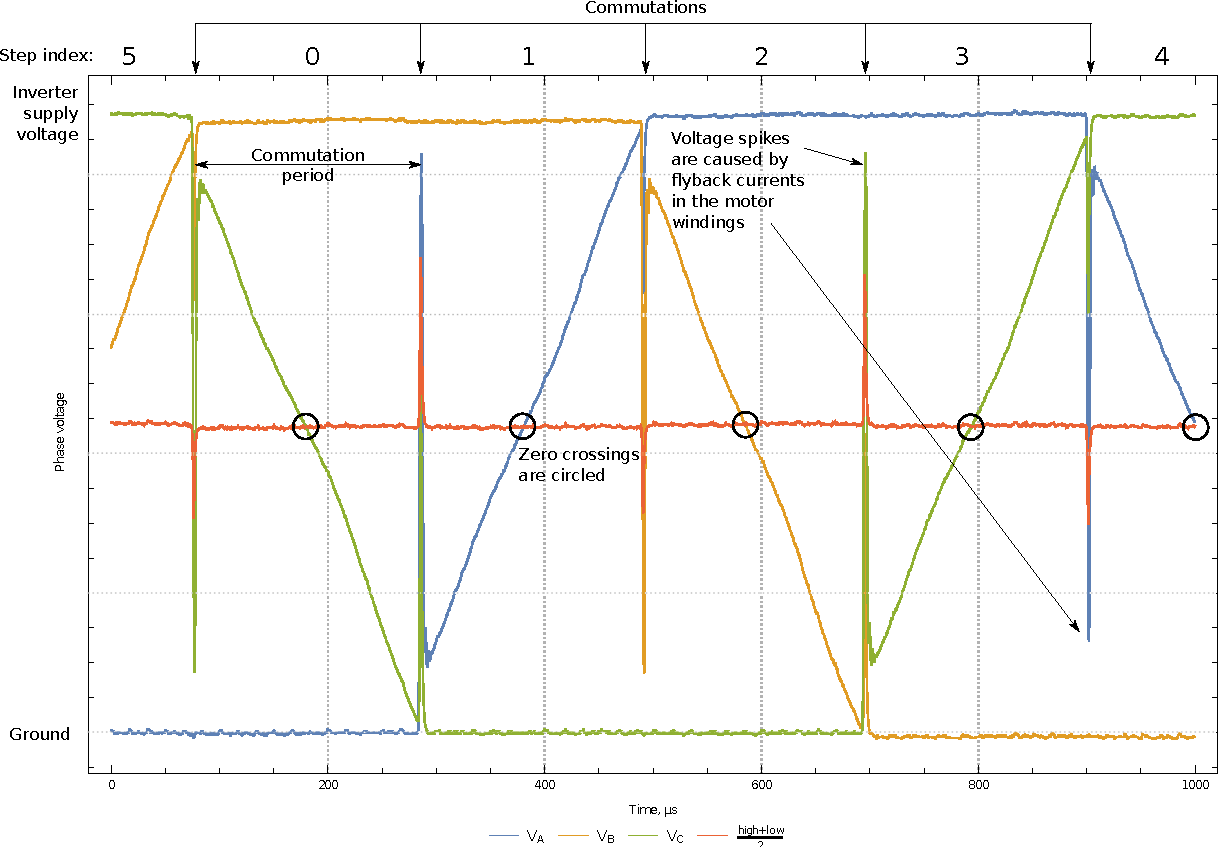
\includegraphics[width=\textwidth]{commutation_basics}
	\caption{Commutation basics.\label{commutation_basics}}
\end{figure}
\begin{figure}[hb]
    \centering
	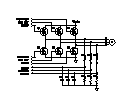
\includegraphics[width=\textwidth]{power_stage_schematic}
	\caption{Commutation basics.\label{power_stage_schematic}}
\end{figure}
\begin{figure}[hb]
    \centering
	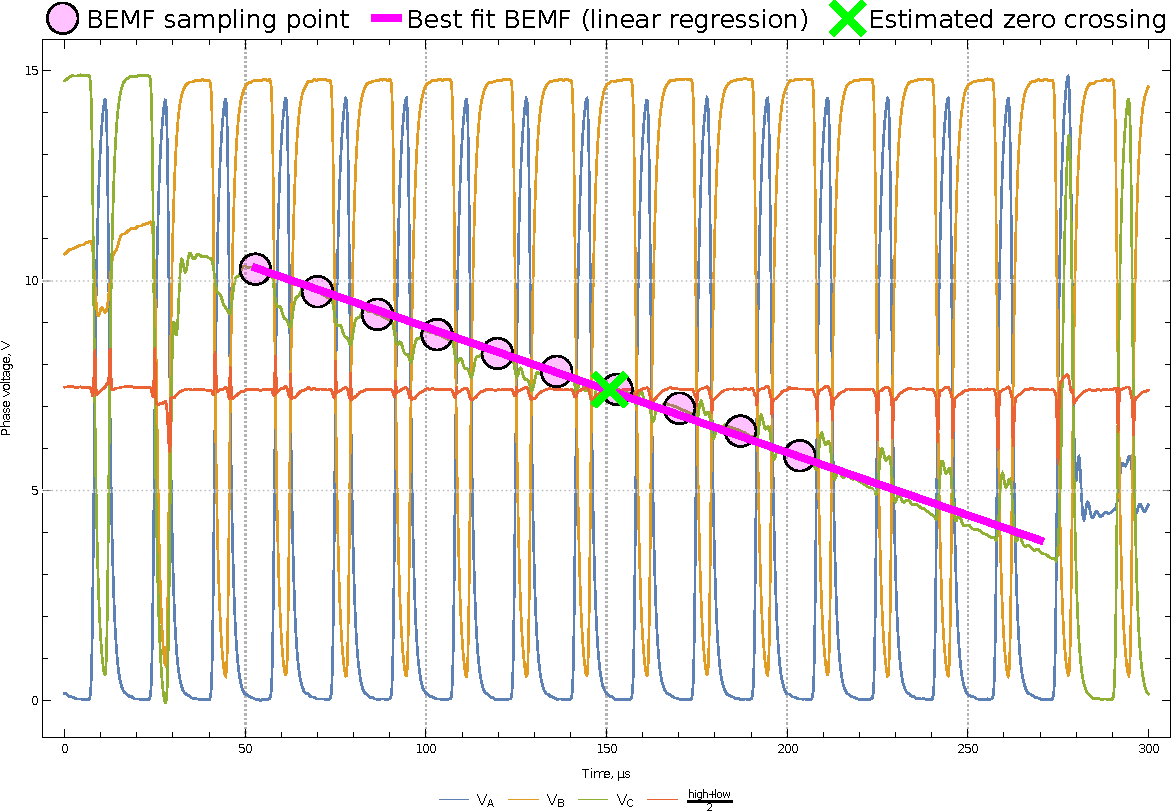
\includegraphics[width=\textwidth]{phase_voltage_sampling}
	\caption{Commutation basics.\label{phase_voltage_sampling}}
\end{figure}
\begin{figure}[hb]
    \centering
	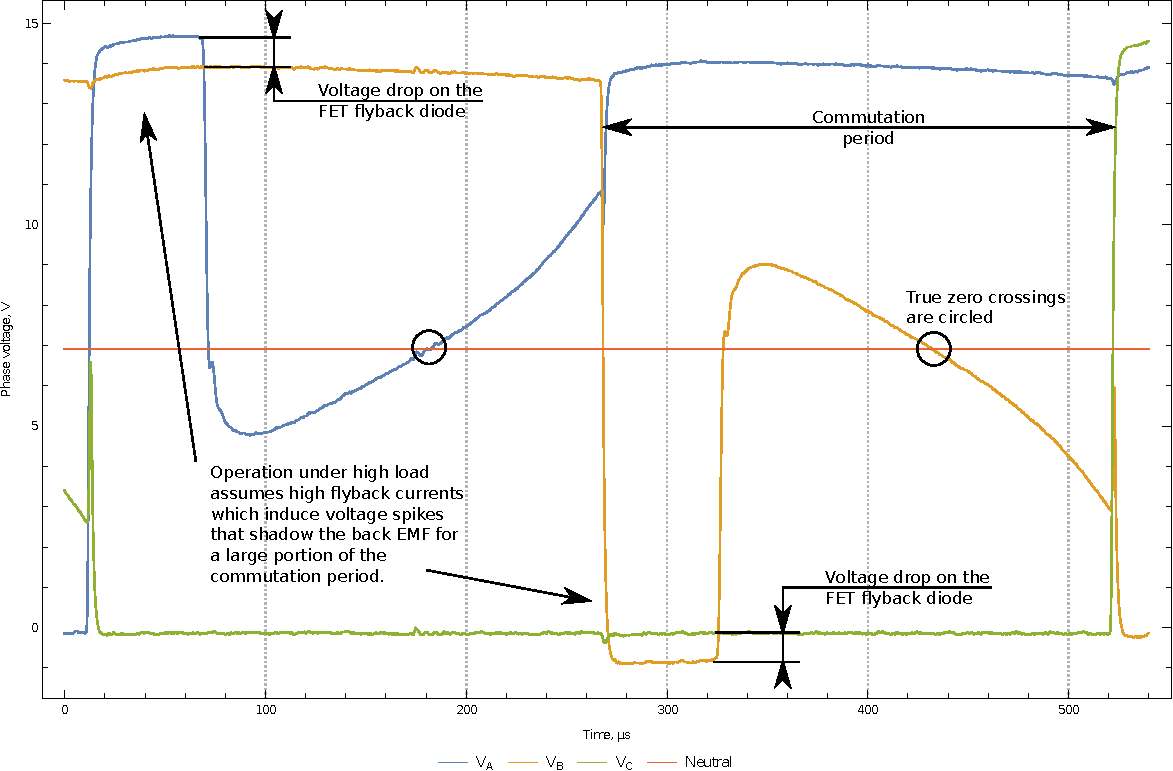
\includegraphics[width=\textwidth]{phase_voltages_at_high_load}
	\caption{Commutation basics.\label{phase_voltages_at_high_load}}
\end{figure}
\begin{figure}[hb]
    \centering
	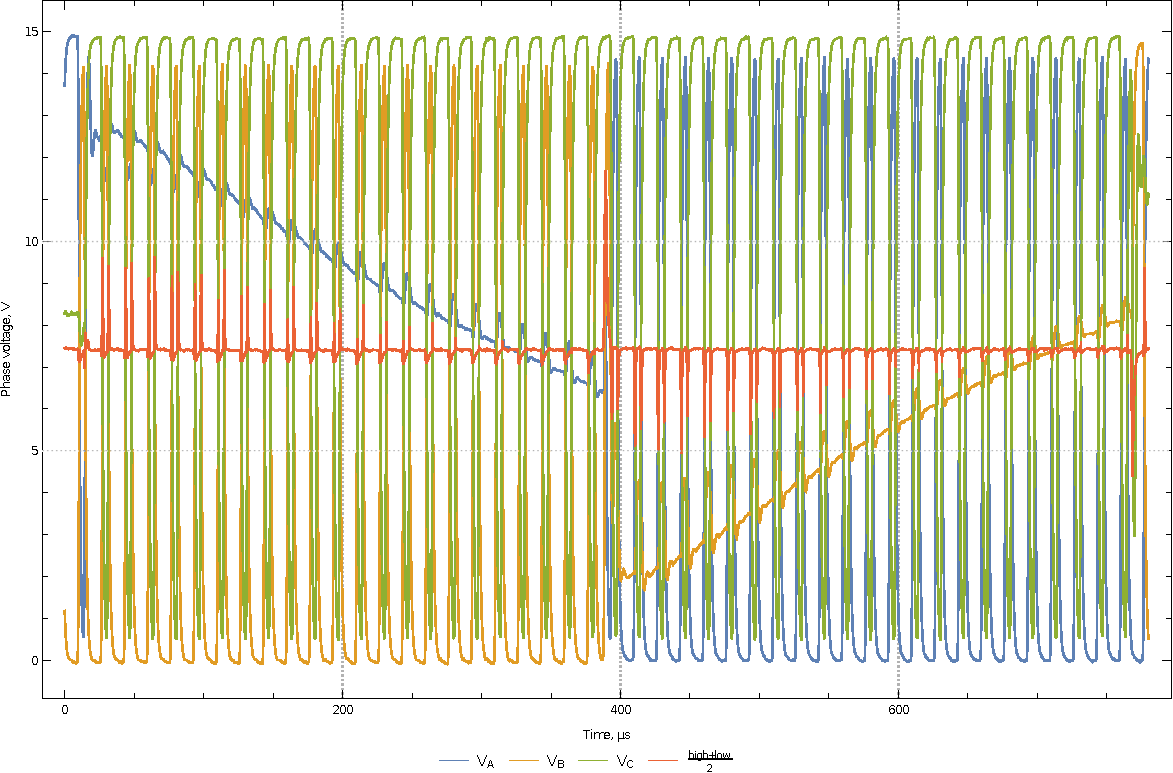
\includegraphics[width=\textwidth]{phase_voltages_at_high_advance_angle}
	\caption{Commutation basics.\label{phase_voltages_at_high_advance_angle}}
\end{figure}
\begin{figure}[hb]
    \centering
	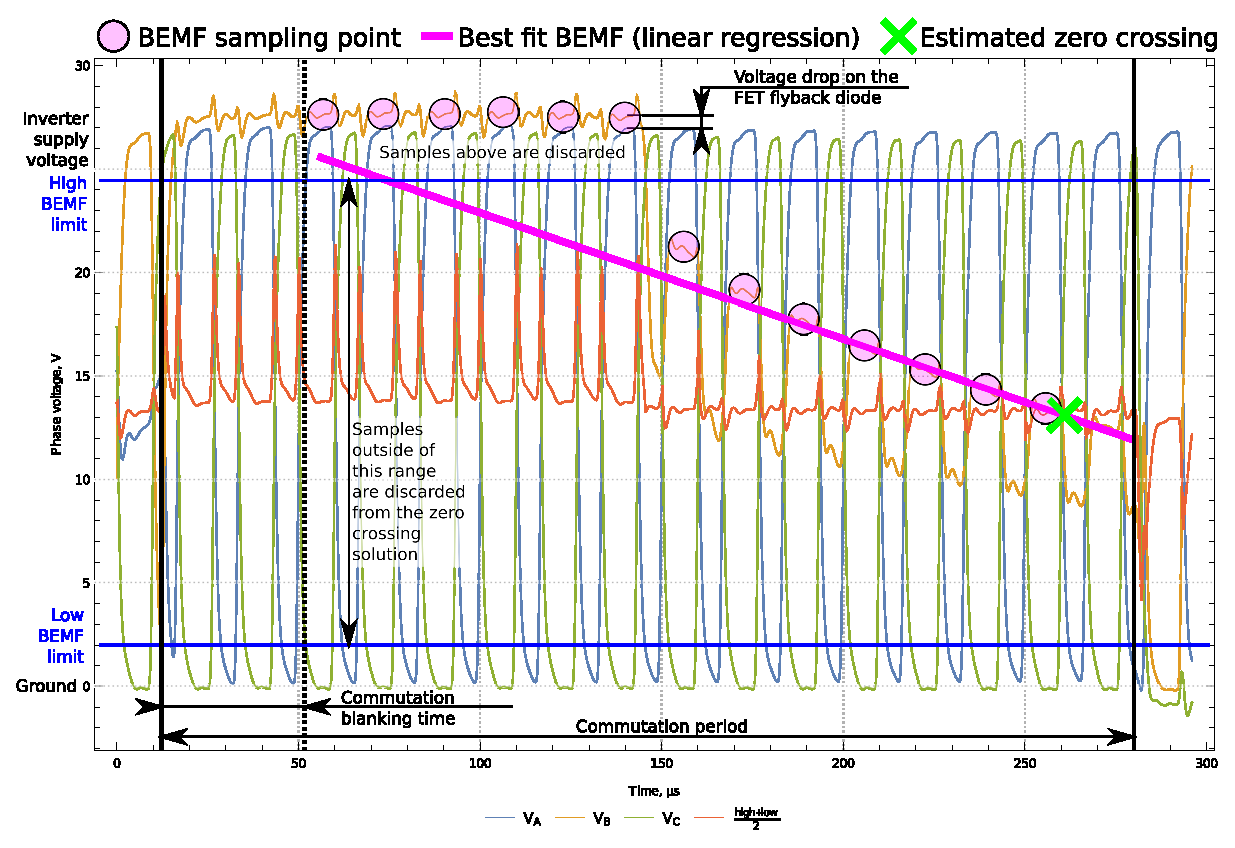
\includegraphics[width=\textwidth]{phase_voltages_braking_high_advance_angle}
	\caption{Commutation basics.\label{phase_voltages_braking_high_advance_angle}}
\end{figure}

\end{document}
